\chapter{Physical Simulations}\label{chapter:physical-simulations}
Modeling the world around us is a longstanding problem of science. For many
physical processes, model equations exist, describing how a given system evolves
through time. From weather and climate forecasts (\cite{stocker2014climate})
over quantum physics (\cite{QuantumSim}), to the control of plasma fusion
(\cite{PlasmaControl}), or optimizing the shape of
vehicles (\cite{OptimizationCFD}), it has become an integral part of engineering
applications to use numerical methods to derive solutions from model equations.

In this section, we build up an understanding of modeling physical phenomena
with \acfp{PDE}. We also introduce the notion of \acf{DP} after a brief
introduction to classical numerical methods.

\section{Partial Differential Equations}
\acp{PDE} are the most fundamental description of evolving systems from quantum
mechanics to turbulent flows. \acp{PDE} are equations relating the partial
derivatives of some unknown function. For a physical system $\vb{u}(\vb{x},t)$,
the governing \ac{PDE} can be written as

\begin{equation}
\label{eq:pde}
\pdv{\vb{u}}{t} = \mathcal{P}\left(\vb{u}, \pdv{\vb{u}}{\vb{x}},
\pdv[2]{\vb{u}}{\vb{x}},\dots,\vb{y}(t)\right),
\end{equation}
where $\mathcal{P}$ models the physical behavior of the system, and $\vb{y}(t)$
denotes an (optional) external force factor. 

\subsection{Numerical Methods}
Analytic solutions (i.e. closed-form expressions) can be found usually only for
very simple \acfp{PDE}. 

\todo{Write only about things that come up later on:}
\todo{
  Numerical Integration:
  \begin{itemize}
    \item Euler Step
    \item Midpoint
    \item RK4
  \end{itemize}
  Finite Differences:
  \begin{itemize}
    \item Replace domain by a finite number of discrete points.
    \item These points are typically located on Eulerian grid.
    \item Discretization: Central difference gives approximation of derivatives.
  \end{itemize}
  $\left( \pdv{q}{x}\right)_i = \frac{q_{i+1} - q_{i-1}}{2\Delta x}$
  ($\pdv{q}{x}$ at grid point $i$) $\rightarrow$ staggered grid: 
  $\left( \pdv{q}{x}\right)_i = \frac{q_{i+1/2} - q_{i-1/2}}{2\Delta x}$
    Finite Elements: (Is the Eigenfluid simulation a Finite Elements method?)
  \begin{itemize}
    \item Replace infinite dimensional solution space by a finite dimensional
      solution space
    \item Function space is constructed by decomposing domain into a set of
      "finite elements" and defining interpolation functions for them
  \end{itemize}
  $\to$ Finite number of unknowns
}

\section{Differentiable Physics}
Given $\vb{u}(\vb{x}, t)$, described by a \ac{PDE} as in Equation~\eqref{eq:pde}, a regular
solver can move the system forward in time via Euler steps:

$$\vb{u}(\vb{x},t) = \text{Solver}\left[ \vb{u}(t_i), \vb{y}(t_i) = 
  \vb{u}(t_i) + \Delta t \cdot \mathcal{P} \left( 
    \vb{u}(t_i), \dots, \vb{y}(t_i)
  \right)
\right],$$

computing a solution trajectory $\vb{u}(t)$, that approximates a solution to the
\ac{PDE}. Although this computation is differentiable, it is not well-suited to
solve optimization problems, since gradients can only be approximated by finite
differencing, and (especially for high-dimensional or continuous systems), this
method would become computationally expensive, because a full trajectory needs
to be computed for each optimizable parameter.

\cite{holl2019pdecontrol} address this issue via the use of differentiable
solvers, backpropagating through the chain of operations via analytic
derivatives.  Differentiable solvers can efficiently compute the derivatives
with respect to any of the inputs $\pdv*{\vb{u}(t_{i+1})}{\vb{u}(t_i)}$ and
$\pdv*{\vb{u}(t_{i+1})}{\vb{y}(t_i)}$. 

\todo{Refer to frameworks already mentioned in section 1.1.2 Differentiable
Solvers. We tried out difftaichi, wasp, and phiflow, then implemented everything
with phiflow. Maybe mention this maybe later on?}

For a basic comparison of the characteristics of supervised and differentiable
physics approaches, see Figure~\ref{fig:learning-to-throw}.

\todo{Rewriting this explanation, and shorten the figure description.}

\subsection{Loss Functions for Differentiable Physics}
\label{dp-loss}
\todo{Observation loss at end step should match target observation.}

\todo{Give only a high-level (mathematical) overview, and hatch it out more in
the problem statement part later on.}

\subsection{Comparison with Supervised Learning}
Figure~\ref{fig:learning-to-throw} shows us the results of a comparison between
teaching the same network with the same objective function, the only difference
being teaching in a supervised and a \ac{DP} manner.  Both the supervised and
the differentiable physics network approximate the function
$f^{-1}(\vb{x_{final}}): \mathbb{R} \mapsto \mathbb{R}^4$, which is the inverse
of the function $f(\vb{x}, \vb{y}, \vb{v}, \vb{\alpha})$, mapping the final
position $\vb{x_{final}}$ of an object being thrown from position $(\vb{x},
\vb{y})$, with velocity $\vb{v}$ and angle $\vb{\alpha}$. The same network
architecture is used, with the weights initialized to the same initial values.
Both networks have seen the same number of training examples, and are using an
$L_2$ norm between the point of impact resulting from the predicted initial
values and the intended position. It is evident that the DP network is able to
get orders of magnitude closer than the supervised network, which has no
knowledge of the underlying physical system, and it's best guess is to
interpolate between the closest data it has seen during training, which results
in a coarse approximation. Also, as the result space to this problem is not
unimodal (i.e. it has multiple possible right answers), the supervised model is
further thrown off, and will give values that are an average of examples seen
during training. This means that even if we increase the training data, the
supervised model can never learn this problem properly.  
\todo{Finalize this description, and refer to where this comes up in our
experiments.}

\begin{figure}
  \centering
  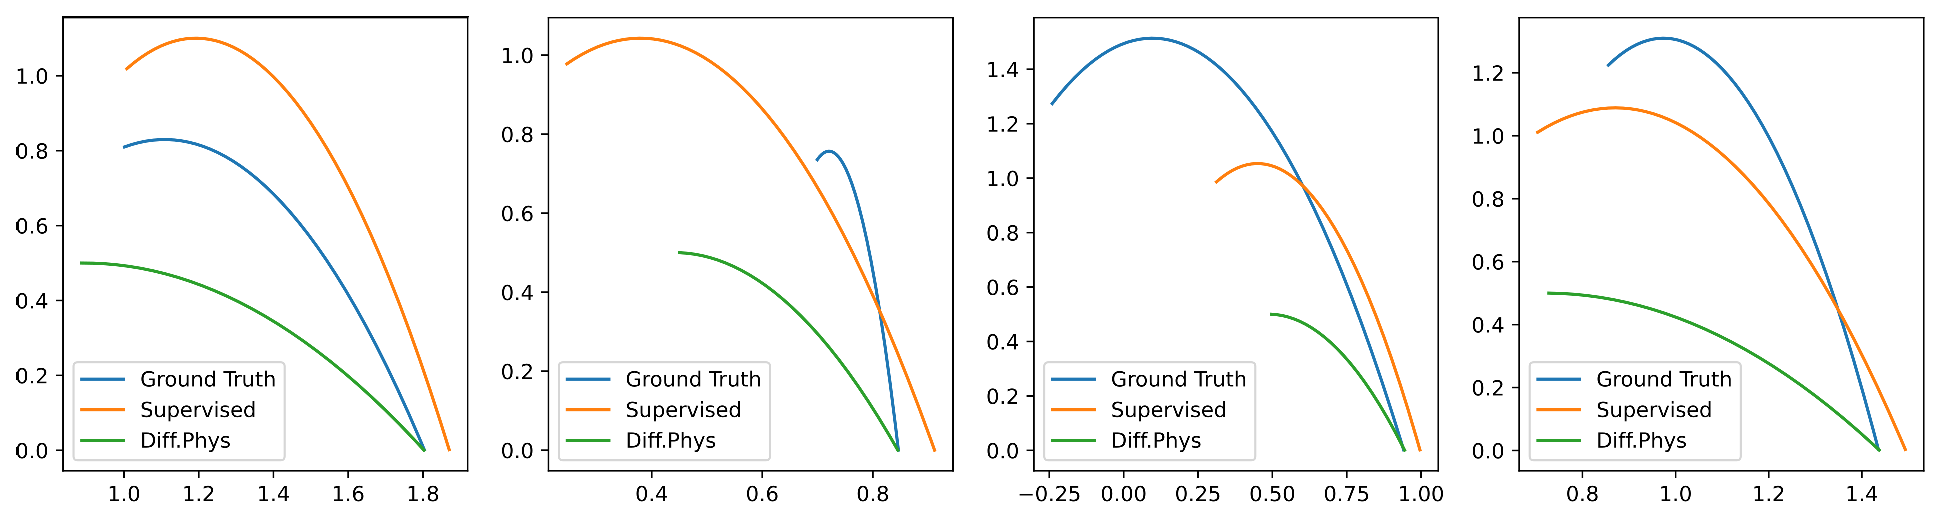
\includegraphics[width=\textwidth]{figures/throwing_results}
  \caption{Learning to throw. The goal is to give an initial velocity $v$, angle
    $\alpha$, and position $\vb{x}$ for a projectile, that hits a target at the
    ground floor when simulated.  The supervised network is outperformed by the
    \ac{DP} approach, as it always hits closer to the target by orders of
    magnitude than its supervised counterpart.  The only difference between the
    two agents being the way they derive their gradients from the same $L_2$
    error: while the \ac{DP} network gains an understanding of the underlying
    physical system via gradients of the simulation, the supervised network only
    sees examples of input-output pairs, where multimodality becomes an inherent
    problem.  (Figure recreated after [\cite{LearnToThrow}].)
  }
    \label{fig:learning-to-throw}
\end{figure}
